\documentclass[10pt,letterpaper,twocolumn]{article}

\usepackage[margin=0.62in]{geometry}
\usepackage[T1]{fontenc}
\usepackage[utf8]{inputenc}
\usepackage{amsmath,amssymb}
\usepackage{booktabs}
\usepackage{enumitem}
\usepackage[dvipsnames]{xcolor}
\usepackage{tikz}
\usepackage{hyperref}
\usetikzlibrary{arrows.meta,positioning,fit,calc,shapes.geometric}

\hypersetup{
  colorlinks=true,
  urlcolor=NavyBlue,
  linkcolor=NavyBlue
}

\setlength{\columnsep}{0.22in}
\setlength{\parindent}{0pt}
\setlength{\parskip}{3pt}
\raggedbottom

\tikzset{
  block/.style={
    draw=MidnightBlue,
    rounded corners=2pt,
    thick,
    fill=MidnightBlue!5,
    align=center,
    minimum height=8mm,
    minimum width=22mm,
    inner sep=4pt
  },
  block2/.style={
    draw=ForestGreen!70!black,
    rounded corners=2pt,
    thick,
    fill=ForestGreen!7,
    align=center,
    minimum height=8mm,
    minimum width=22mm,
    inner sep=4pt
  },
  block3/.style={
    draw=BrickRed,
    rounded corners=2pt,
    thick,
    fill=BrickRed!7,
    align=center,
    minimum height=8mm,
    minimum width=22mm,
    inner sep=4pt
  },
  line/.style={-{Latex[length=2.2mm]}, thick, draw=black!70},
  dashedline/.style={-{Latex[length=2.2mm]}, thick, dashed, draw=black!55},
  smallnote/.style={font=\footnotesize, align=center}
}

\title{\textbf{d\_model: Agentic Autoresearch for Task-Conditioned Robot Co-Design}}
\author{Repo-grounded technical note for \texttt{IL\_ideation}}
\date{April 19, 2026}

\begin{document}
\maketitle

\begin{abstract}
This note distills the architecture implemented in the current \texttt{IL\_ideation} repository into a compact systems paper. The central idea is not ``ask a model for a better robot,'' but rather place proposal models inside a bounded robotics search loop. The codebase combines structured candidate generation, deterministic task conditioning, render/BOM/telemetry validation, a single human approval checkpoint via \texttt{program.md}, and a remote trial loop that edits morphology and controller code, trains a graph neural controller, rolls out the design in MuJoCo, and scores outcomes with both simulator metrics and a Gemini ER-style success oracle. The resulting stack is best understood as a hybrid agentic co-design framework: language models propose, deterministic components constrain, simulation measures, and the system keeps only improvements that survive execution.
\end{abstract}

\section{Introduction}

Robotics design pipelines usually separate embodiment selection from controller learning. A human chooses a morphology, hand-builds a simulator representation, and only then begins policy optimization. This repository tries to compress those stages into a unified co-design loop: describe a task, generate viable robot candidates, ground them into engineering artifacts, approve a research agenda once, and iterate both body and controller under measured feedback.

That distinction matters because it separates \emph{prompt chaining} from \emph{autoresearch}. In prompt chaining, a language model is repeatedly asked for a better answer. In autoresearch, a proposal is executed, scored, and either retained or discarded. The codebase is explicitly structured around the second pattern. Proposal models appear in candidate generation and code editing, but they are surrounded by hardrails, ranking logic, validation checks, and trial execution.

\begin{figure*}[t]
\centering
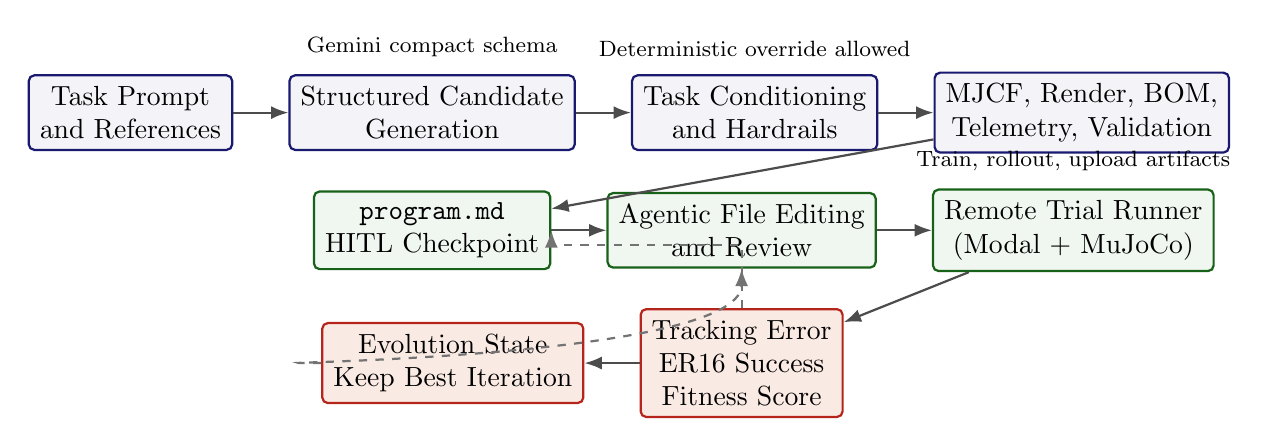
\begin{tikzpicture}[node distance=5mm and 7mm]
\node[block] (task) {Task Prompt\\and References};
\node[block, right=of task] (gen) {Structured Candidate\\Generation};
\node[block, right=of gen] (rank) {Task Conditioning\\and Hardrails};
\node[block, right=of rank] (art) {MJCF, Render, BOM,\\Telemetry, Validation};
\node[block2, below=of gen] (program) {\texttt{program.md}\\HITL Checkpoint};
\node[block2, right=of program] (agent) {Agentic File Editing\\and Review};
\node[block2, right=of agent] (modal) {Remote Trial Runner\\(Modal + MuJoCo)};
\node[block3, below=of agent] (score) {Tracking Error\\ER16 Success\\Fitness Score};
\node[block3, left=of score] (best) {Evolution State\\Keep Best Iteration};

\draw[line] (task) -- (gen);
\draw[line] (gen) -- (rank);
\draw[line] (rank) -- (art);
\draw[line] (art) -- (program);
\draw[line] (program) -- (agent);
\draw[line] (agent) -- (modal);
\draw[line] (modal) -- (score);
\draw[line] (score) -- (best);
\draw[dashedline] (best.west) .. controls +(180:18mm) and +(270:12mm) .. (agent.south);
\draw[dashedline] (score.north) -- ++(0,8mm) -| (program.east);

\node[smallnote, above=1mm of gen] {Gemini compact schema};
\node[smallnote, above=1mm of rank] {Deterministic override allowed};
\node[smallnote, above=1mm of modal] {Train, rollout, upload artifacts};
\end{tikzpicture}
\caption{System architecture implemented or directly scaffolded in the repository. Proposal, control, and execution are separated rather than conflated into one model call.}
\label{fig:system}
\end{figure*}

\section{System Overview}

Figure~\ref{fig:system} shows the repository's full stack. The front half of the system is already concrete: task interpretation, robot candidate generation, capability-based reranking, and engineering artifact synthesis. The back half is the autoresearch loop: a user-approved \texttt{program.md}, bounded code editing, remote trial execution, and keep-best evolution state.

Two design decisions are especially important. First, the generation API uses a deliberately compact provider-facing schema. The repository documents that richer schemas can fail under Gemini structured outputs due to state explosion, so generation emits a smaller contract and reconstructs richer internal objects deterministically afterward. Second, the model's preferred design can be overridden by rule-based task conditioning, which prevents a plausible-looking but task-misaligned candidate from dominating the search.

\section{Agentic Architecture}

The agentic portion of the system is implemented as a constrained coding loop rather than a general autonomous assistant. The orchestrator has three explicit jobs:

\begin{enumerate}[leftmargin=4mm,itemsep=1pt]
\item Draft \texttt{program.md} from the task plan so the human approves the search agenda once.
\item Edit only designated files, typically morphology and training code, from a prompt plus current file contents.
\item Review generated PyTorch code for device-placement mistakes before execution.
\end{enumerate}

This is a practical architecture. Human input is centralized at the agenda level; low-level iteration is automated afterward. The system therefore reduces approval overhead without removing human control over the objective.

\begin{figure}[t]
\centering
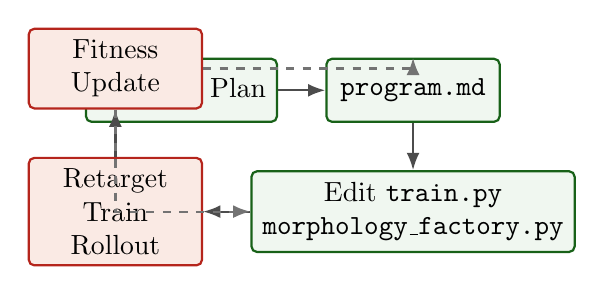
\begin{tikzpicture}[node distance=6mm and 6mm]
\node[block2] (plan) {ER-style Plan};
\node[block2, right=of plan] (prog) {\texttt{program.md}};
\node[block2, below=of prog] (edit) {Edit \texttt{train.py}\\\texttt{morphology\_factory.py}};
\node[block3, left=of edit] (trial) {Retarget\\Train\\Rollout};
\node[block3, above=of trial] (fit) {Fitness\\Update};

\draw[line] (plan) -- (prog);
\draw[line] (prog) -- (edit);
\draw[line] (edit) -- (trial);
\draw[line] (trial) -- (fit);
\draw[dashedline] (fit) |- (edit);
\draw[dashedline] (fit) -| (prog);
\end{tikzpicture}
\caption{Autoresearch loop: agenda, edit, execute, score, and iterate. The model proposes edits, but the loop is closed by execution and fitness, not by text alone.}
\label{fig:loop}
\end{figure}

The operational flow is:

\begin{enumerate}[leftmargin=4mm,itemsep=1pt]
\item read editable files into context,
\item prompt the model for full-file replacements,
\item apply only named outputs back to disk,
\item launch a remote trial,
\item record the returned fitness and artifacts,
\item mark the best iteration in the evolution state.
\end{enumerate}

This gives the repository an agentic architecture with clear boundaries: the model is never the source of truth for state, metrics, or artifact quality. The store, validator, and trial runner are.

\section{DL Framework}

The deep learning stack is intentionally small but well targeted.

\subsection{Morphology latent model}

The morphology module defines a 12-dimensional parameterization over continuous values such as torso length, arm length, leg length, damping, stiffness, and friction, plus discrete values such as limb counts and degrees of freedom. A VAE maps this design space into an 8-dimensional latent:

\begin{equation}
\mathcal{L}_{\text{VAE}}(x)=\lVert x-\hat{x}\rVert_2^2 + \beta D_{KL}\left(q_\phi(z|x)\,\|\,\mathcal{N}(0,I)\right).
\end{equation}

The encoder and decoder both use hidden width 64. Methodologically, the VAE acts as a compressive prior over robot morphologies, enabling guided sampling and reusable local structure instead of unconstrained random search.

\subsection{Morphology-agnostic graph controller}

The controller is more distinctive. Instead of binding control to a single robot body, the repository constructs a graph directly from MJCF:

\begin{itemize}[leftmargin=4mm,itemsep=1pt]
\item nodes correspond to MuJoCo bodies,
\item edges correspond to bidirectional joint relations,
\item node features have dimension 16,
\item edge features have dimension 6 and encode joint type plus axis.
\end{itemize}

These features are encoded and passed through three GATv2-based message-passing layers with head counts $(4,4,1)$ and hidden size 64. A linear decoder then emits a scalar output per node. In compact form:

\begin{equation}
h^{(0)}_v=W_n x_v,\quad e_{uv}=W_e a_{uv},
\end{equation}
\begin{equation}
h^{(\ell+1)}=\mathrm{GATv2}\!\left(h^{(\ell)}, E, e\right),\;\ell\in\{1,2,3\},
\end{equation}
\begin{equation}
\hat{u}_v = W_o h^{(3)}_v.
\end{equation}

The important property is weight sharing across morphologies. The same controller class can be trained on different body graphs without redefining the network architecture.

\begin{figure}[t]
\centering
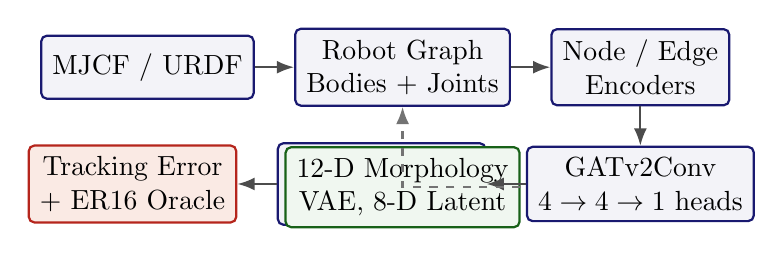
\begin{tikzpicture}[node distance=5mm and 5mm]
\node[block] (mjcf) {MJCF / URDF};
\node[block, right=of mjcf] (graph) {Robot Graph\\Bodies + Joints};
\node[block, right=of graph] (enc) {Node / Edge\\Encoders};
\node[block, below=of enc] (gat) {GATv2Conv\\$4 \rightarrow 4 \rightarrow 1$ heads};
\node[block, left=of gat] (dec) {Linear Decoder\\Scalar / Node};
\node[block3, left=of dec] (loss) {Tracking Error\\+ ER16 Oracle};
\node[block2, below=of graph] (vae) {12-D Morphology\\VAE, 8-D Latent};

\draw[line] (mjcf) -- (graph);
\draw[line] (graph) -- (enc);
\draw[line] (enc) -- (gat);
\draw[line] (gat) -- (dec);
\draw[line] (dec) -- (loss);
\draw[dashedline] (vae.east) -| (graph.south);
\end{tikzpicture}
\caption{DL stack: a morphology prior proposes bodies while a graph controller consumes the resulting body graph. Evaluation combines simulator tracking and a vision-language success estimate.}
\label{fig:dl}
\end{figure}

\subsection{Hybrid fitness}

The trial runner does not optimize on a purely differentiable reward. It retargets motion to a sampled morphology, trains in MuJoCo, rolls out a replay, and then computes fitness from both tracking error and an ER16-style success probability estimated from the replay video. This is a hybrid objective: one term is simulator-native and one term is oracle-mediated. The benefit is broader task semantics; the cost is added variance and dependence on external model quality.

\section{Methodology}

The repository's methodology is best described as \emph{hybrid agentic co-design}. It mixes learned, symbolic, and operational components instead of forcing every decision through a single model.

\subsection{Task-conditioned selection}

The first methodological anchor is that task language is converted into explicit capability requirements before final candidate choice. The task-conditioning layer builds a capability graph with required affordances such as payload stability, traction strategy, low-profile clearance, dual-arm grasping, or surface attachment. Candidates are then evaluated against those capabilities, annotated with missing requirements and risk flags, and reranked even when the proposal model prefers a different design.

This is more important than it may seem. A plain multimodal model can generate a coherent robot description that is locally plausible but globally mismatched to the task. By translating free-form task descriptions into capability checks, the repository inserts an explicit semantic bottleneck between proposal and selection.

\begin{table}[t]
\centering
\small
\begin{tabular}{@{}lll@{}}
\toprule
Layer & Mechanism & Role \\
\midrule
Proposal & Gemini structured output & diverse candidates, code edits \\
Selection & task graph + hardrails & deterministic reranking \\
Grounding & MJCF / GLB / BOM / telemetry & inspection artifacts \\
Learning & VAE + GNN controller & body prior and policy \\
Execution & Modal + MuJoCo & run and score trials \\
Human control & \texttt{program.md} & approve research agenda \\
\bottomrule
\end{tabular}
\caption{Methodological decomposition of the repo. The point is not one perfect model, but a layered loop with explicit responsibilities.}
\label{tab:layers}
\end{table}

One concrete example is candidate scoring. The implementation combines capability coverage, design quality, and model confidence, adds a small embodiment prior, and subtracts risk penalties:

\begin{equation}
s(c)=0.7\,\kappa(c)+0.25\,q(c)+0.05\,p(c)+0.05\,\mathbf{1}[e(c)\in E^\star]-0.15\,r(c).
\end{equation}

Hardrail failure can cap the score to a low ceiling before final selection. This means search is not left to model preference alone.

Another methodological strength is artifact grounding. Candidate designs are validated for structural consistency, task fit, compiler outputs, render richness, simulation viability, and procurement confidence. Even when some telemetry is heuristic rather than measured on hardware, the system still produces a far more falsifiable record than plain text generation.

\subsection{Validation and operator review}

The validation stage is not just a logging pass. It functions as an intermediate engineering filter between design generation and expensive iterative search. Structural completeness rejects impossible limb and torso combinations; compiler checks require usable MJCF and GLB outputs; render checks enforce minimum richness for inspection use; procurement checks ensure the design is grounded enough to support a build plan; and telemetry exposes likely control bottlenecks before a user approves the agenda.

This is also where the repository's human factors become clear. The operator is shown summarized, stable artifacts rather than raw model prose. In practical terms, that makes the system easier to review, easier to challenge, and easier to keep aligned with engineering intent.

\section{Current Limits}

The repository should be read carefully. Its strongest realized contribution is the front half of the co-design stack: structured proposal, deterministic reranking, inspection artifacts, and operator workflow. The end-to-end evolution loop is architecturally present and reasonably concrete, but its quality still depends on deployed Modal workers, Supabase storage, MuJoCo runtime, and access to Gemini models.

There is also an epistemic limit in the evaluation strategy. The ER16-style oracle expands the system's semantic reach, but it introduces dependence on a model-based judge. Likewise, cost, backlash, and bandwidth estimates are useful review heuristics rather than hardware-calibrated measurements. This does not invalidate the approach, but it does mean the current repository is best understood as a local-first robotics research workspace rather than a finished robot compiler.

\section{Conclusion}

\texttt{IL\_ideation} is most interesting when framed as a layered autoresearch system for robot co-design. The proposal model is only one component. Deterministic task conditioning keeps the search honest, artifact generation makes candidates inspectable, a graph controller allows cross-morphology control, a morphology VAE provides a compact body prior, and the remote trial runner closes the loop with measured execution. In short: the repository treats robot design the way autoresearch treats model improvement---as a search problem over proposals that must survive real evaluation.

\end{document}
